%% NSS-MIC_Instructions.tex
%% 8/2007
%% By Bo Yu (yu@bnl.gov)
%% based on:
%% bare_jrnl.tex
%% V1.3
%% 2007/01/11
%% by Michael Shell
%% see http://www.michaelshell.org/
%% for current contact information.
%%
%% This is a skeleton file demonstrating the use of IEEEtran.cls
%% (requires IEEEtran.cls version 1.7 or later) with an IEEE journal paper.
%%
%% Support sites:
%% http://www.michaelshell.org/tex/ieeetran/
%% http://www.ctan.org/tex-archive/macros/latex/contrib/IEEEtran/
%% and
%% http://www.ieee.org/


%%*************************************************************************
%% Legal Notice:
%% This code is offered as-is without any warranty either expressed or
%% implied; without even the implied warranty of MERCHANTABILITY or
%% FITNESS FOR A PARTICULAR PURPOSE!
%% User assumes all risk.
%% In no event shall IEEE or any contributor to this code be liable for
%% any damages or losses, including, but not limited to, incidental,
%% consequential, or any other damages, resulting from the use or misuse
%% of any information contained here.
%%
%% All comments are the opinions of their respective authors and are not
%% necessarily endorsed by the IEEE.
%%
%% This work is distributed under the LaTeX Project Public License (LPPL)
%% ( http://www.latex-project.org/ ) version 1.3, and may be freely used,
%% distributed and modified. A copy of the LPPL, version 1.3, is included
%% in the base LaTeX documentation of all distributions of LaTeX released
%% 2003/12/01 or later.
%% Retain all contribution notices and credits.
%% ** Modified files should be clearly indicated as such, including  **
%% ** renaming them and changing author support contact information. **
%%
%% File list of work: IEEEtran.cls, IEEEtran_HOWTO.pdf, bare_adv.tex,
%%                    bare_conf.tex, bare_jrnl.tex, bare_jrnl_compsoc.tex
%%*************************************************************************
\documentclass[journal]{IEEEtran}
\usepackage{graphicx}

\begin{document}
\title{Software reliability: Experiences\\
in European scientific research\\
projects and new trends}
%
% author names and IEEE memberships
% note positions of commas and nonbreaking spaces ( ~ ) LaTeX will not break
% a structure at a ~ so this keeps an author's name from being broken across
% two lines.
% use \thanks{} to gain access to the first footnote area
% a separate \thanks must be used for each paragraph as LaTeX2e's \thanks
% was not built to handle multiple paragraphs
%

\author{D.C. Duma, %~\IEEEmembership{Member,~IEEE,}
        E. Ronchieri, %~\IEEEmembership{Fellow,~OSA,}
        P. Orviz Fernandez, %~\IEEEmembership{Life~Fellow,~IEEE}% <-this % stops a space
        M. David, %~\IEEEmembership{Life~Fellow,~IEEE}% <-this % stops a space
        J. Gomes, %~\IEEEmembership{Life~Fellow,~IEEE}% <-this % stops a space
        D. Salomoni %~\IEEEmembership{Life~Fellow,~IEEE}% <-this % stops a space
\thanks{D. C. Duma, E. Ronchieri, and D. Salomoni are with INFN - CNAF, Bologna, Italy.}%
\thanks{P. Orviz Fernandez, is with CSIC, Santander, Spain, (e-mail: orviz@ifca.unican.es)}%
\thanks{M. David, and J. Gomes are with LIP, Lisbon, Portugal}%
}

\maketitle
\pagestyle{empty}
\thispagestyle{empty}

\begin{abstract}
In this work we describe the trends in scientific software reliability by analyzing past European Commission funded software development projects in the context of distributed computing field, such as Enabling Grids for E-sciencE, European Middleware Initiative and the ongoing INDIGO-DataCloud.
\end{abstract}

%\begin{IEEEkeywords}
%IEEEtran, journal, \LaTeX, paper, template.
%\end{IEEEkeywords}


\section{Evolution of Software Reliability}
% The very first letter is a 2 line initial drop letter followed
% by the rest of the first word in caps.
%
% form to use if the first word consists of a single letter:
% \IEEEPARstart{A}{demo} file is ....
%
% form to use if you need the single drop letter followed by
% normal text (unknown if ever used by IEEE):
% \IEEEPARstart{A}{}demo file is ....
%
% Some journals put the first two words in caps:
% \IEEEPARstart{T}{his demo} file is ....
%
% Here we have the typical use of a "T" for an initial drop letter
% and "HIS" in caps to complete the first word.

\IEEEPARstart{I}{n} the European scientific research arena, the analysis of some of the last decade software development projects depicts a continuous increase of the prominence and robustness of testing and validation procedures. The observed trends are aligned with the evolution of the software engineering techniques (e.g. rise of DevOps practices \cite{devops}) over the last years. This is tied to the parallel advancements in the ICT field (with virtualization and container technologies) and the advent of automation and event-response tools. In the following we introduce a set of European Commission funded projects, starting in 2001 up to now, where the authors were and are currently involved. For each project we explain how they addressed the challenge in software reliability.

\begin{figure*}
\centering
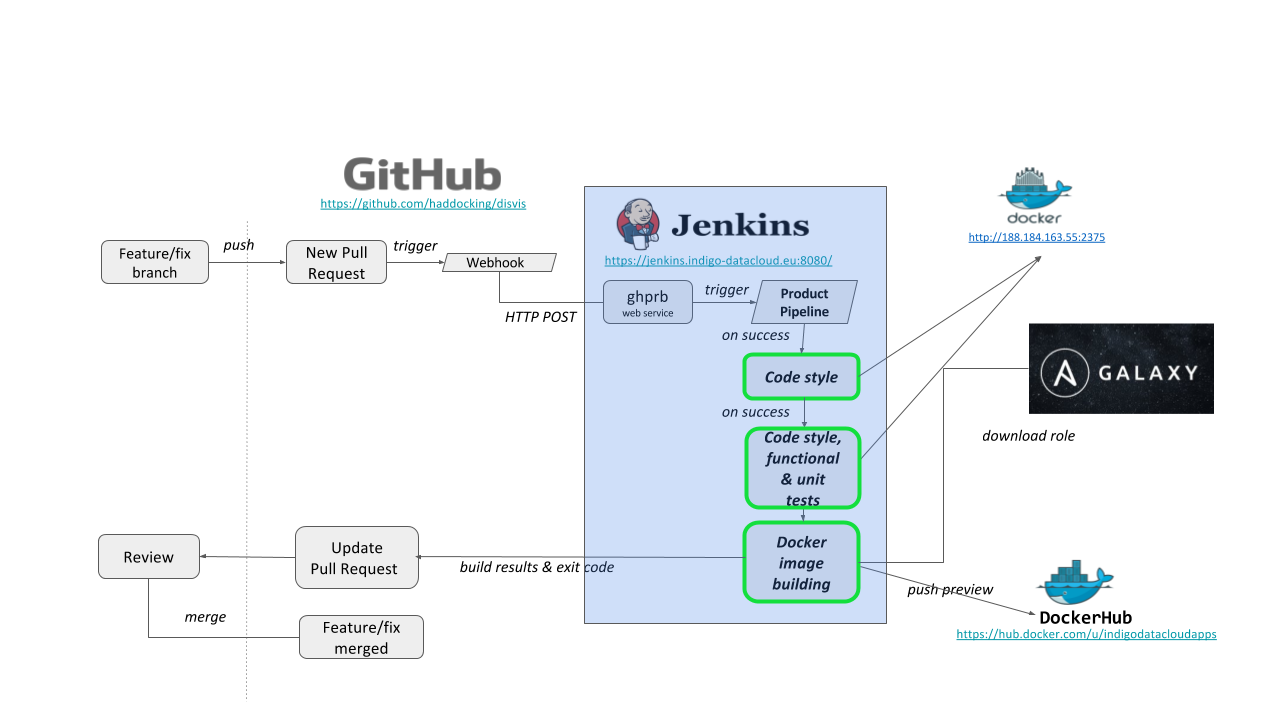
\includegraphics[width=\textwidth]{images/devops.png}
\caption{Continuous Delivery workflow for Docker images.}
\label{fig:fig_CD}
\end{figure*}

The DataGrid \cite{cordis:datagrid} project (Jan 2001 -- Dec 2003) was devoted to develop software to provide Grid computing functionalities and related management tools for widely distributed scientific communities, such as the Large Hadron Collider (LHC) experiments, Earth observations and Bioinformatics. In this project, a large effort was dedicated in the definition and implementation of academic software engineering practices due to the unusual context in which DataGrid aims, starting from the large geographical distribution of the teams involved in the development tasks, evolving requirements coming from the different application areas and the design of a new technology: the Grid \cite{datagrid}. DataGrid developed its own software distribution, {\sl EDG} (European DataGrid), strongly based on Globus Middleware Services \cite{globus}. An Architecture Task Force coordinated the overall design and technical consistency of the developments, complemented by the definition of various testing phases: preparation, execution and documentation.

The three phases of Enabling Grids for E--sciencE (EGEE, Apr 2004 -- Apr 2010) \cite{cordis:egee, cordis:egee2, cordis:egee3} projects brought together scientists and engineers from more than 240 institutions in 45 countries worldwide to provide a seamless Grid infrastructure for e--Science, available 24 hours--a--day. One of the main achievements of these projects was the middleware -- a crucial component of any Grid infrastructure as it provides the {\sl glue} that links the hardware resources within such infrastructure. The {\sl gLite} middleware \cite{glite} was the ultimate official distribution of EGEE as of 2006, after two years of prototyping and re--engineering efforts to converge with LHC Computing Grid ({\sl LCG-2}), Virtual Data Toolkit ({\sl VDT}) and {\sl Condor} \cite{condor} software distributions. The overall goal of the middleware engineering group was to provide and maintain selected middleware services of the {\sl gLite} distribution to satisfy the needs of the scientific communities. During EGEE--I, a software process was designed and put into action for the early releases of the {\sl gLite} middleware. This release process favoured a development environment of rapidly changing interfaces that were necessary during re--engineering. Starting in EGEE--II, there was a need to move to a more dynamic release process, and the first steps were taken towards an automated environment. At this stage  no software metrics were collected, while functional and integration testing were performed manually, and only on the last project, EGEE--III, an automatic build system was adopted; the E--Infrastructure for Testing, Integration and Configuration of Software ({\sl ETICS}) service. The {\sl gLite} middleware developed within EGEE will evolve further as part of a new project: the European Middleware Initiative (EMI).

The ETICS \cite{cordis:etics} and ETICS 2 \cite{cordis:etics2} (Jan 2006 -- Feb 2010) projects aimed at defining and implementing a framework able to integrate a combination of new technologies in test management, release management tools and resource virtualization to improve quality, reliability and interoperability of large--scale scientific software. Both projects supported mechanisms to measure static software metrics (such as Lines of Code (LOC), Source LOC (SLOC), and Complexity); to measure the number of faults, the number of defects, number of bugs; execute unit testing; deploy and test software on a virtual set of resources \cite{etics}. The {\sl ETICS} portal was the first automated service for delivering software products in distributed environments such as the Grid.

The EMI (May 2010 -- Apr 2013) project \cite{cordis:emi} aimed to deliver a consolidated set of middleware products based on the four major middleware providers in Europe -- {\sl ARC}, {\sl dCache}, {\sl gLite} and {\sl UNICORE}. The EMI Quality Model used ISO/IEC 9126 Software Engineering -- Product Quality Standard \cite{iso9126} to identify a set of characteristics that need to be present in EMI software products and processes to be able to meet EMI quality requirements. For each software characteristic, a set of associated metrics and Key Performance Indicators (KPIs) were identified and defined in detail in the EMI Metrics Specification \cite{emi-metrics}. EMI was one of the first projects in using a Continuous Integration (CI) system for building, packaging and testing the various components. It leveraged the {\sl ETICS} tool and its plugin framework that provided not only the ability of collecting metrics during build and test execution, but also to make queries on the collected data and chart them through its chart generation framework.

The EGI--InSPIRE (Integrated Sustainable Pan--European Infrastructure for Researchers in Europe, May 2010 -- May 2014) project \cite{cordis:egi-inspire} is the continuation of EGEE--III project, establishing and maintaining a sustainable European Grid Infrastructure. EGI--InSPIRE did not develop any software but maintained a production--ready Grid computing middleware distribution called {\sl UMD} (Unified Middleware Distribution). The role of {\sl UMD} was to enforce the fulfilment of a set of quality criteria definitions \cite{egi-qc} in the software being delivered (i.e., {\sl EMI} and {\sl Globus}) \cite{mario}. {\sl UMD} is still being used and deployed in the European scientific e--Infrastructures as a result of its continuation under a follow--up project, the EGI--Engage (Engaging the EGI Community towards an Open Science Commons) \cite{cordis:egi-engage}. This distribution is currently complemented by a Cloud--specific one called {\sl CMD} (Cloud Middleware Distribution).

\begin{figure*}
\centering
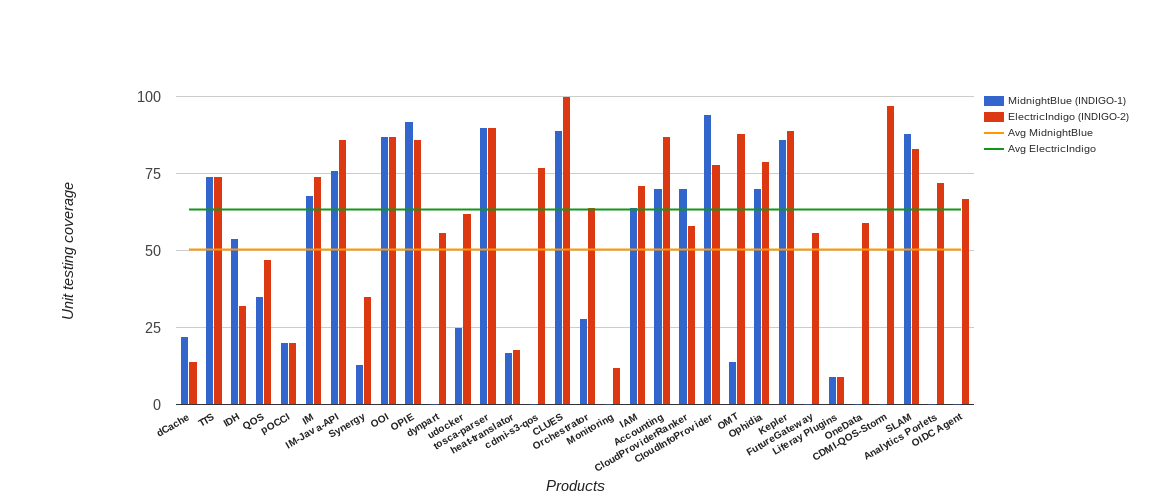
\includegraphics[width=\textwidth]{images/unittest.png}
\caption{Unit testing coverage for the two major INDIGO--DataCloud releases.}
\label{fig:fig_unittest}
\end{figure*}

INDIGO--DataCloud (INtegrating Distributed data Infrastructures for Global ExplOitation) \cite{cordis:indigo} is an ongoing software development project that started on April $1^{st}$ 2015 with the aim at providing solutions to address the existing gaps in the three cloud levels; IaaS, PaaS and SaaS, helping developers, e--Infrastructures and scientific communities to exploit cloud computing resources. The project will end on September 2017.

\section{New Trends in Software Reliability}

The INDIGO--Datacloud project is a reflection of the progress made in software quality and reliability aspects throughout the past scientific European experiences. Nevertheless, the project’s Quality Assurance procedures are also highly influenced by the insights of current big worldwide collaborations of software development. These collaborations have continuously inspired new technologies and procedures to increase the robustness and quality of the software being delivered. In this scenario, the DevOps culture is one of the major outcomes that has been progressively adopted in the INDIGO--DataCloud project.

\subsection{DevOps practices}

The DevOps methods emphasize on exercising Quality Assurance techniques to avoid infrastructure disruption whenever new developments are deployed into production. The INDIGO--DataCloud project promoted the application of a CI scenario to enforce the Quality Assurance requirements for any piece of software being produced within the project. Such environment requires an automated ready--to--go infrastructure where the different services involved (source code management platform, automation server) interact with each other to trigger the quality check execution and return back the exit codes, together with their outputs. To accomplish this, the project leveraged tightly integrated open source tools such as GitHub and Jenkins, as well as relying on Docker container provisioning to speed up the source code validation. This CI approach is guiding the project’s software development phase throughout the first and second major releases.

As DevOps suggests, frequent releases positively affects the reliability of the software. The software updates of INDIGO--DataCloud products taking place since the second major release are passing through a Continuous Delivery (CD) pipeline that adds the packaging of the software right after the execution of the quality checks (as part of the CI). The steps defined within the CD pipeline differ whether the software is to be distributed in the form of Docker images or via operating system’s packages. In the latter case an extra validation step is added, consisting in the product’s deployment using a Configuration Management (CM) solution. The installation uses the packages being built in the previous step, which are being uploaded to a testing repository. In the case of Docker images, the CM is used to build the image itself, installing and configuring the product before uploading it to the DockerHub repository \cite{indigo-dockerhub}. Figure \ref{fig:fig_CD} showcases the workflow followed by the products distributed as Docker images.

\subsection{Software Quality Procedures}

The software quality procedures \cite{indigo-d31} cover: 1) the identification and description of the \emph{quality requirements} that the software need to comply with, and 2) the \emph{quality metrics}.

The requirements are applied at early stages in the software development process, integrated in the Jenkins CI service \cite{indigo-jenkins}, so any bug or design issue is likely to be detected and corrected promptly. The source code is publicly available in GitHub repositories under an organization called {\sl indigo-dc} \cite{indigo-github} to augment the visibility of the product catalogue, promoting the external contributions and software adoption. In this regard, the source code is compliant with community de--facto style standards, selected from the variety of programming languages being used.

\begin{figure}[!t]
\centering
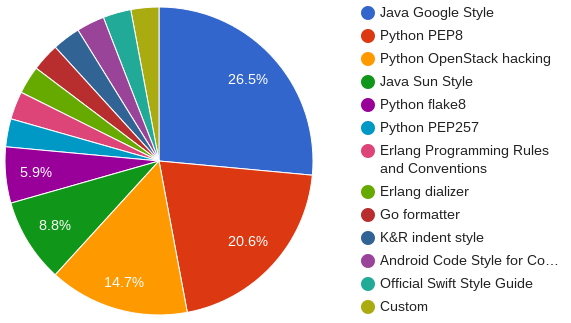
\includegraphics[width=0.5\textwidth]{images/codestyle.png}
\caption{Code style standards followed by INDIGO--DataCloud's software products.}
\label{fig:fig_codestyle}
\end{figure}

Tests are triggered in each build to measure the unit and functional testing coverage, with a recommended value of 70\% of coverage in the former case. The documentation of the products is treated as source code, using a markup language, automatically rendered and uploaded in online repositories \cite{indigo-gitbook}. Changes in both documentation and source code are human--reviewed as the last step before merging them into the production repository. Last but not least, as already seen in the DevOps section, in order to facilitate the usage of the INDIGO--DataCloud services, they can be deployed automatically using either Ansible \cite{indigo-ansible} or Puppet \cite{indigo-puppet} open--source tools.

The evaluation of the software quality is performed by measuring the values of the metrics and Key Performance Indicators (KPIs) defined based upon the ISO/IEC 9126 Software engineering -- Product quality standard. These metrics cover the development, release and maintenance phases of the software lifecycle. Development and release metrics are obtained automatically from several sources, such as GitHub and Jenkins CI service, and graphically displayed as GitHub pages using GrimoireLab framework \cite{grimoirelab}. Maintenance and user support metrics are collected from the different sources of data like GGUS \cite{ggus} and Github Issues.

\subsection{Integration, preview and early adoption}

Two pilot infrastructures are at the disposal of developers and scientific communities involved in the project. The aim of these testbeds is to test the level of integration between the components involved in the INDIGO--DataCloud solution and use cases validation, by deploying and executing the applications with the last stable version of the software.

The released software is also tested in production environments through the stage--rollout process. Selected resource providers are requested to install the most updated stable versions of the software, accessed by their users. The stage--rollout process is key to detect and mitigate issues that could only appear in production.

\section{Conclusion}

It is a fact that the European software produced for scientific purposes is evolving to a more sustainable model where the quality and reliability of software is being prioritized. Recent software engineering insights, such as DevOps, are gradually being applied as the open--source collaborative tools evolve, allowing tighter integrations. The focus of the Software Quality Assurance procedures has been integrated in the development stage, trying to detect and correct issues early in the software lifecycle. Automation and metric analysis are at the base of prompt issue solving. However, post--release validation, such as integration testbeds and the stage--rollout process, are also needed to strengthen the software reliability for scientific usage.

%\appendices
%\section{}
%Appendices, if needed, appear before the acknowledgment.

% use section* for acknowledgement
\section*{Acknowledgment}
The authors would like to thanks European Commission with the various funded projects.


% references section

% can use a bibliography generated by BibTeX as a .bbl file
% BibTeX documentation can be easily obtained at:
% http://www.ctan.org/tex-archive/biblio/bibtex/contrib/doc/
% The IEEEtran BibTeX style support page is at:
% http://www.michaelshell.org/tex/ieeetran/bibtex/
%\bibliographystyle{IEEEtran}
% argument is your BibTeX string definitions and bibliography database(s)
%\bibliography{IEEEabrv,../bib/paper}
%
% <OR> manually copy in the resultant .bbl file
% set second argument of \begin to the number of references
% (used to reserve space for the reference number labels box)
\begin{thebibliography}{1}

\bibitem{devops}
M. Walls, \emph{Building a DevOps Culture}, in O'Reilly Media, 1 edition (April 15, 2013)

\bibitem{cordis:datagrid}
\emph{DataGrid project}, European Community Research and Development Information Service (CORDIS). Available: http://cordis.europa.eu/project/rcn/53665\_en.html

\bibitem{datagrid}
[3] L. Momtahan, A. Martin, \emph{e-Science Experiences: Software Engineering Practice and the EU DataGrid}, in Proc. Asia-Pacific Software Engineering Conference, Gold Coast, Queensland, Australia, 4-6 Dec. 2002, pp. 269-275, IEEE Press

\bibitem{globus}
I. Foster, C. Kesselman, \emph{Globus: a Metacomputing Infrastructure Toolkit}, International Journal of Supercomputer Applications, vol. 11, no. 2, pp. 115–128, 1997

\bibitem{cordis:egee}
\emph{Enabling Grids for E-sciencE (EGEE)} project, European Community Research and Development Information Service (CORDIS). Available: http://cordis.europa.eu/project/rcn/80149\_en.html

\bibitem{cordis:egee2}
\emph{Enabling Grids for E-sciencE-II (EGEE-II)} project, European Community Research and Development Information Service (CORDIS). Available: http://cordis.europa.eu/project/rcn/99189\_en.html

\bibitem{cordis:egee3}
\emph{Enabling Grids for E-sciencE-III (EGEE-III)} project, European Community Research and Development Information Service (CORDIS). Available: http://cordis.europa.eu/project/rcn/87264\_en.html

\bibitem{glite}
E. Laure et al, \emph{Programming the Grid with gLite}, in Jin, H., Reed, D.A., Jiang, W. (eds.) Computational Methods in Science and Technology, vol. 12(1), pp. 33–45, 2006, Scientific Publishers OWN

\bibitem{condor}
D. Thain, T. Tannenbaum, M. Livny, \emph{Condor and the grid}, in Grid Computing: Making the Global Infrastructure a Reality, Chapter 11, pp. 63–70, 2002, Eds. John Wiley \& Sons Inc.

\bibitem{cordis:etics}
\emph{E-Infrastructure for Testing, Integration and Configuration of Software (ETICS)} project, European Community Research and Development Information Service (CORDIS). Available: http://cordis.europa.eu/project/rcn/80138\_en.html

\bibitem{cordis:etics2}
\emph{E-Infrastructure for Testing, Integration and Configuration of Software - Phase 2 (ETICS 2)} project, European Community Research and Development Information Service (CORDIS). Available: http://cordis.europa.eu/project/rcn/86604\_en.html

\bibitem{etics}
A. Di Meglio, M.-E.Bégin, P. Couvares, E. Ronchieri, E. Takacs, \emph{ETICS: the international software engineering service for the grid}, in Journal of Physics: Conference Series, Vol. 119, N. 4, 2008, IOP Publishing Ltd

\bibitem{cordis:emi}
\emph{European Middleware Initiative (EMI)} project, European Community Research and Development Information Service (CORDIS). Available: http://cordis.europa.eu/project/rcn/95311\_en.html

\bibitem{iso9126}
\emph{ISO/IEC 9126 Software Engineering - Product Quality}, International Organization for Standarization. Available: https://www.iso.org/standard/22749.html

\bibitem{emi-metrics}
\emph{EMI Metrics Specification}. Available: https://goo.gl/LdS6fL

\bibitem{cordis:egi-inspire}
\emph{European Grid Initiative: Integrated Sustainable Pan-European Infrastructure for Researchers in Europe (EGI-InSPIRE)} project, European Community Research and Development Information Service (CORDIS). Available: http://cordis.europa.eu/project/rcn/95923\_en.html

\bibitem{egi-qc}
\emph{EGI Quality Criteriai}. Available: http://egi-qc.github.io/

\bibitem{mario}
M. David et al, \emph{Validation of Grid Middleware for the European Grid Infrastructure}, in Journal of Grid Computing, vol. 12, issue 3, pp. 543–558, 2014, Springer

\bibitem{cordis:egi-engage}
\emph{Engaging the EGI Community towards an Open Science Commons (EGI-ENGAGE)} project, European Community Research and Development Information Service (CORDIS). Available: http://cordis.europa.eu/project/rcn/194937\_en.html

\bibitem{cordis:indigo}
\emph{INtegrating Distributed data Infrastructures for Global ExplOitation (INDIGO-DataCloud)} project, European Community Research and Development Information Service (CORDIS). Available: http://cordis.europa.eu/project/rcn/194882\_en.html

\bibitem{indigo-dockerhub}
\emph{INDIGO-DataCloud DockerHub repository}. Available: https://hub.docker.com/u/indigodatacloud

\bibitem{indigo-d31}
\emph{Initial Plan for WP3} INDIGO-DataCloud Deliverable 3.1. Available: https://www.indigo-datacloud.eu/documents/initial-plan-wp3-d31

\bibitem{indigo-jenkins}
\emph{INDIGO-DataCloud Jenkins CI service}. Available: https://jenkins.indigo-datacloud.eu:8080/

\bibitem{indigo-github}
\emph{INDIGO-DataCloud GitHub Source Code repository}. Available: https://www.github.com/indigo-dc

\bibitem{indigo-gitbook}
\emph{INDIGO-DataCloud GitBook Documentation repository}. Available: https://www.gitbook.com/@indigo-dc

\bibitem{indigo-puppet}
\emph{INDIGO-DataCloud PuppetForge repository}. Available: https://forge.puppet.com/indigodc

\bibitem{indigo-ansible}
\emph{INDIGO-DataCloud Ansible Galaxy repository}. Available: https://galaxy.ansible.com/indigo-dc/

\bibitem{grimoirelab}
\emph{GrimoireLab}. Available: http://grimoirelab.github.io/

\bibitem{ggus}
\emph{Global Grid User Support (GGUS)}. Available: https://www.ggus.eu/

\end{thebibliography}



% that's all folks
\end{document}


